\documentclass[pss]{wiley2sp} % provides pss two-column style
\usepackage{amsmath}
\usepackage{subfig}

\renewcommand{\arraystretch}{1.2} % please do not remove or change
\tolerance=400
\emergencystretch=10pt

\begin{document}

% Title of the article
\title{Optical spin injection, current injection, and second-harmonic
generation in hydrogenated graphene structures}

% Authors
\author{
    Reinaldo Zapata-Pe\~na\textsuperscript{\Ast,\textsf{\bfseries 1}},
    Sean M. Anderson\textsuperscript{\Ast,\textsf{\bfseries 1}},
    Bernardo S. Mendoza\textsuperscript{\Ast,\textsf{\bfseries 1}},
    Anatoli I. Shkrebtii\textsuperscript{\textsf{\bfseries 2}}}

% Abbreviated list of authors for the page headers
\titlerunning{Optical spin injection, current injection, and SHG study of
hydrogenated graphene}
\authorrunning{R. Zapata-Pe\~na et al.}

%E-mail-address of corresponding author
\mail{e-mail
  \textsf{bms@cio.mx}, Phone:
  +52-477-441-4200, Fax: +52-477-441-4209}

% author's affiliations/addresses
\institute{%
  \textsuperscript{1}\,Centro de Investigaciones en \'Optica, Le\'on,
  Guanajuato 37150, M\'exico\\
  \textsuperscript{2}\,University of Ontario, Institute of Technology, Oshawa,
  ON, L1H 7L7, Canada}

\received{XXXX, revised XXXX, accepted XXXX}
\published{XXXX} % do not change, will be filled in by the publisher

% Please select about four verbal keywords for your manuscript.
\keywords{graphene, spin polarization, current injection, second-harmonic.}

\abstract{%
\abstcol{%
We present a theoretical study of spin and current injection, and 
second-harmonic generation via optical means from the C$_{16}$H$_{8}$-alt and
C$_{16}$H$_{8}$-up graphene structures. The incidence of circularly polarized
light onto nonmagnetic semiconductors produces spin-polarized electrons in the
conduction bands. Current injection and second-harmonic generation are
nonlinear, second-order effects that can be produced from both the bulk and
surface of non-centrosymmetric materials. In centrosymmetric materials, these
effects can only be observed at the surface where the inversion symmetry is
broken.} {We also report results for the degree of spin polarization, current
injection, and second-harmonic generation calculated within a full electronic
band structure scheme at the DFT-LDA level using a planewave basis. Our
results show that these effects can be optically generated in both the
C$_{16}$H$_{8}$-alt and C$_{16}$H$_{8}$-up structures, presenting an
anisotropic behavior. We obtain a maximum degree of spin polarization of 39\%
for C$_{16}$H$_{8}$-alt, and 57\% for C$_{16}$H$_{8}$-up, which are
promising results for potential applications in spintronics.}}

\maketitle


\section{Introduction}\label{sec:intro}

Graphene is an allotrope of carbon with a planar, hexagonal, two-dimensional
honeycomb structure with one carbon atom at each vertex \cite{geim2007rise}.
Graphene has attracted great interest due to its distinctive physical
properties, such as the fractional quantum Hall effect, optical absorption,
thermal conductivity, and band structure \cite{geim2007rise,nair2008fine}.
Graphene can be produced via several techniques, the most common of these is
graphite exfoliation for producing small graphene sheets. Larger graphene
films on the order of centimeters obtained by chemical vapor deposition on
copper substrates using methane.

Graphene has been characterized with a variety of microscopic and mechanical
techniques such as atomic force microscopy, transmission electron microscopy,
scanning tunneling microscopy, and Raman spectroscopy
\cite{geim2007rise,rao2009graphene,boehm1994nomenclature,novoselov2005two}.
Graphene behaves like a metal \cite{geim2007rise} but its band gap can be
tuned by changing the total area \cite{han2007energy}, applying an electric
field \cite{zhang2009direct}, or by doping \cite{ohta2006controlling,%
elias2009control,guisinger2009exposure,samarakoon2010tunable}. This paper
presents a study on two hydrogenated graphene structures. We can obtain
different spatial configurations by varying the amount and location of the
hydrogen doping. As shown in Fig. \ref{fig:structures}, when a H atom is
bonded to a carbon atom in the graphene plane, it pulls the carbon atom from
the plane modifying the carbon-carbon bond length, and possibly opening the
band gap \cite{samarakoon2010tunable}. The C$_{16}$H$_{8}$-alt and
C$_{16}$H$_{8}$-up systems presented in this paper both have 50\%
hydrogenation and present a band gap.

We focus on three phenomena used for characterizing semiconducting systems:
the degree of spin polarization (DSP), optical current injection (OCI), and 
second-harmonic generation (SHG). The optical spin injection is characterized by 
the adimensional degree of spin polarization (DSP), which is a function of
frequency. The DSP is the fraction of injected electrons in the conduction
bands that are spin polarized versus those that are not. There are theoretical
reports of DSP calculations for bulk media (Si, GaAs, CdSe, and Ge
semiconductors) \cite{nastos2007full,cabellos2009stress,rioux2010optical} and
surfaces [Si(111):In, Si(111):As, GaAs(110):Sb, GaAs(110), and Si(111) with
$4\times2$ and $8\times2$ reconstructions]
\cite{mendoza2012optical,arzate2014optical}.

The OCI is a surface-sensitive optical effect with potential application for surface characterization and chemical reaction control. It is a second-order nonlinear process that takes place in non-centrosymmetric materials \cite{nastos2006optical,cabellos2011optical,bhat2005excitonic,fraser1999quantum}. This photocurrent has been studied in bulk semiconductors \cite{atanasov1996coherent,sipe2000second}, one dimensional (1D) nanotubes \cite{mele2000coherent,kral2000photogalvanic}, and two dimensional (2D) surfaces \cite{mele2000coherent,cabellos2011optical}.

Nonlinear optical spectroscopies, particularly SHG, are important methods for
styudying surface properties due to their noninvasive and nondestructive
nature. These properties include atomic structure, phase transitions,
adsorption of atoms, and many others \cite{dadap1997second,%
daum1993identification,mcgilp1994probing,power1995resonant,%
godefroy1996electric,salazar2014molecular,chen1981surface,%
mendoza1998microscopic}. 
SHG is a particular case of the nonlinear optical process of sum of frequency in which photons of same frequency are annihilated to produce a new photon with twice the frequency and energy and half of the wavelength of the initial photons. This phenomena occurs when light beams from coherent sources inside over a nonlinear media that does not present inversion of symmetry \cite{bloembergen1962light,andersonPRB15,sipe2000second}.

The organization of the sections of this paper is as follows. In Sec.
\ref{sec:theory} we present the theory and formulas that describe the DSP,
current injection, and SHG. In Sec. \ref{sec:results} we describe the details
of the calculation and the corresponding spectra for the respective \emph{alt}
and \emph{up} structures. Finally, we give our conclusions in Sec.
\ref{sec:conclusions}.


\section{Theory}\label{sec:theory}

\begin{changed}
In this section we present the formulas used for calculating the DSP \cite{nastos2007full,mendoza2012optical}, OCI \cite{cabellos2011optical,sipe2000second}, and SHG \cite{andersonPRB15}. For a full derivations see the references for each.
\end{changed}

\begin{figure}[t]
\subfloat[Top and side view of C$_{16}$H$_{8}$-alt.]
{\includegraphics[width=\linewidth]{alt/altstruct1}}
\hfill
\subfloat[Top and side view of C$_{16}$H$_{8}$-up.]
{\includegraphics[width=\linewidth]{up/upstruct1}}
\caption{The \emph{alt} and \emph{up} structures. The light
(dark) spheres correspond to hydrogen (carbon) atoms.\label{fig:structures}}
\end{figure}

\subsection{Optical spin injection}

The injection and detection of spin polarized electrons into nonmagnetic
materials is the core of spintronics \cite{vzutic2004spintronics,%
fert2008nobel,pezzoli2012optical,bottegoni2013experimental,%
bottegoni2013photoinduced} and an important problem in condensed matter
theory. The process of optical spin injection appears when circularly
polarized light (CPL) \cite{dyakonov1984theory} is incident on a
semiconducting material. This allows spin polarized electrons to move from the
valence to the conduction bands. This process is the result of the interaction
between the electron spin and the motion caused by the spin-orbit coupling in
the material. The DSP is the percentage of injected spin polarized electrons
in the conduction bands. It can be calculated with full band structure local-
density approximation (LDA), and $\textbf{k}\cdot\textbf{p}$ methods
\cite{nastos2007full,cabellos2009stress}.

The spin and carrier generation rate can be described by 

\begin{align*}
\dot{S}^{a}(\omega) &= \zeta^{abc}(\omega)E^{b}(-\omega)E^{c}(\omega), \nonumber \\ 
\dot{n}(\omega)     &= \xi^{bc}E^{b}(-\omega)E^{c}(\omega)
\end{align*}
where $\zeta^{abc}$ is the spin injection rate tensor and $\xi^{bc}$ is the carrier generation rate tensor. The spin injection rate tensor is given by
\begin{align}\label{eq:zeta}
\zeta^{abc} &= \frac{i\pi e^{2}}{\hbar^{2}}\int\frac{d^{3}k}{8\pi^{3}}
\sum_{vcc'}^{\prime}\text{Im}\bigl[S^{a}_{c'c}(\textbf{k})
r^{b}_{vc'}(\textbf{k})r^{c}_{cv}(\textbf{k})\nonumber\\
&\qquad+S^{a}_{cc'}(\textbf{k})
r^{b}_{vc}(\textbf{k})r^{c}_{c'v}(\textbf{k})\bigr]
\delta(\omega_{cv}(\textbf{k})-\omega),
\end{align}
where $S^{n}$ and $r^{n}$ are the spin and position matrix elements. The carrier generation rate tensor is related to the linear optical response tensor by $\xi^{bc}$=Im$[(2/\hbar)\chi^{bc}]$ . The $abc$ superscripts denote the Cartesian coordinates and the expression of Eq. \eqref{eq:zeta} satisfies the $\zeta^{abc} = -\zeta^{acb}$ condition.

We assume an incoming beam of CPL at normal incidence that propogates along the $-z$ direction, $\mathbf{E}(\omega) = E_{0}(\omega)(\hat{x} - i\hat{y})/\sqrt{2}$. The DSP along a given $a$ direction is defined as $D^{a}=\dot{S}^{a}(\omega)/(\hbar/2)\dot{n}(\omega)$, which can be reduced to 
\begin{equation}\label{eq:D^i}
D^{a}(\omega) = 
\frac{-4i\zeta^{axy}(\omega)}
    {\hbar\left[\xi^{xx}(\omega) + \xi^{yy}(\omega)\right]}.
\end{equation}

It is generally possible to generate spin-polarized electrons along all three
Cartesian directions. 
% The total DSP can be obtainedas

% \begin{equation*}
% \left|D^{\text{T}}\right| = \sqrt{D_{x}^{2} + D_{y}^{2} + D_{z}^{2}}.
% \end{equation*}


\begin{changed}
\subsection{Optical current injection}

This current can be produced with a single optical beam of CPL via the interference of one photon-absorption processes from different linear polarizations of light \cite{sipe2000second}. The  OCI is defined as
\begin{equation}
\mathbf{\dot{J}}^{a}_{\text{inj}}(\omega) =
\eta^{abc}(\omega)E_{b}(\omega)E_{c}(\omega), \label{eq:eta}
\end{equation}
where $\eta^{abc}(\omega)$ is the surface injection current tensor and is given by
\begin{align*}
\eta(\omega) =  \frac{i\pi e^{3}}{\hbar^{2}}&\int\frac{d^{3}k}{8\pi^{3}}
\nonumber \\
\times &
\sum_{vc}\Delta^{a}_{cv}(\mathbf{k})\text{Im}\big[r^{b}_{cv}(\mathbf{k})
r^{c}_{cv}(\mathbf{k})\big]\delta(\omega_{cv}(\mathbf{k})-\omega).
\end{align*}
$r^{n}$ is the position matrix elements and 
\begin{equation*}
\Delta^{a}_{cv} = v^{a}_{cc}(\mathbf{k})-v^{a}_{vv}(\mathbf{k}),
\end{equation*}
where $v^{a}_{nn}(\mathbf{k})=p^{a}_{nn}(\mathbf{k})/m_{e}$ is the electron velocity for band $n$.

The tensor $\eta^{abc}(\omega)$ is purely imaginary and is antisymmetric with respect to the last two indices, \emph{b} and \emph{c} \cite{sipe2000second,nastos2006optical}. It is possible to generate current injection along all three directions with incident CPL on the surface plane.

% The total injection current can be obtained in a similar way as has been done in Eq. \ref{eq:D^i}

% \begin{equation}
%     \left|{\eta^{\text{T}}}\right| = \sqrt{ \eta_{xxy}^{2} +
%     \eta_{yxy}^{2} + \eta_{zxy}^{2} },
% \end{equation}

\end{changed}


\subsection{Second-harmonic generation}

We follow the derivation developed in reference \cite{andersonPRB15}. This new formalism to calculate the second order susceptibility includes the scissors correction, the contribution of the nonlocal part of the pseudopotentials, and the cut function. 

The second order nonlinear polarization is given by 
\begin{equation*}
\mathcal{P}(2\omega) = \chi^{abc}(-2\omega;\omega,\omega)E^{b}(\omega)E^{c}(\omega)
\end{equation*}
where $\chi^{abc}$ is the nonlinear susceptibility tensor responsible for the SHG and satisfies the $\chi^{abc}$ = $\chi^{acb}$ condition. The superscripts $abc$ denote the Cartesian components.  

The expressions for the imaginary part of $\chi^{abc}$ for the interband (\emph{e}) and intraband (\emph{i}) contributions, at $1\omega$ and $2\omega$ are given by
\begin{subequations}\label{eq:chis}
\begin{align}
\mathrm{Im}[\chi^{\mathrm{a}\mathrm{b}\mathrm{c}}_{e,\omega}] =  
\frac{\pi |e|^3}{2\hbar^2}\int 
&
\frac{dk^3}{8\pi^3}  
\nonumber \\
\times \sum_{vc}\sum_{q\neq(v,c)}
\frac{1}{\omega^\Sigma_{cv}}
&
\left[\frac{\mathrm{Im}[\mathbf{v}^{\Sigma,\mathrm{a}}_{qc}\{r^{\mathrm{b}}_ 
{cv}r^{\mathrm{c}}_{vq}\}]} {(2\omega^\Sigma_{cv}-\omega^\Sigma_{cq})} \right.
\nonumber \\
& 
\left. -\frac{\mathrm{Im}[\mathbf{v}^{\Sigma,\mathrm{a}}_{vq}\{r^{\mathrm{c}}
_{qc}r^{\mathrm{b}}_{cv}\}]} {(2\omega^\Sigma_{cv}-\omega^\Sigma_{qv})}
\right]\delta(\omega^\Sigma_{cv}-\omega),
\end{align}

\begin{align}
\mathrm{Im}  [\chi^{\mathrm{a}\mathrm{b}\mathrm{c}}_{i,\omega}]= 
\frac{\pi\vert e\vert^3}{2\hbar^2}
&
\int \frac{dk^3}{8\pi^3} 
\nonumber \\
 \times \sum_{cv}\frac{1}{(\omega^\Sigma_{cv})^{2}} 
&
\Bigg[
\mathrm{Re}\left[\left\{r^{\mathrm{b}}_{cv}\left(\mathbf{v}^
{\Sigma,\mathrm{a}}_{vc}\right)_{;k^{\mathrm{c}}}\right\}\right]
\nonumber \\
&+\frac{\mathrm{Re}\left[\mathbf{v}^{\Sigma,\mathrm{a}}_{vc}\left\{
r^{\mathrm{b}}_{cv}
\Delta^{\mathrm{c}}_{cv}\right\}\right]}{\omega^\Sigma_{cv}} 
\Bigg]
\delta(\omega^\Sigma_{cv}-\omega),
\end{align}

\begin{align}
\mathrm{Im}[\chi^{\mathrm{a}\mathrm{b}\mathrm{c}}_{e,2\omega}]= -
&
\frac{\pi |e|^3}{2\hbar^2}\int \frac{dk^3}{8\pi^3}
\nonumber \\
\times \sum_{vc}\frac{4}{\omega^\Sigma_{cv}}
&
\Bigg[
\sum_{v'\ne v}\frac{\mathrm{Im}[\mathbf{v}^{\Sigma,\mathrm{a}}_{vc}\{r^{\mathrm{
b}}_{cv'}r^{\mathrm{c}}_{v'v}\}]}
{2\omega^\Sigma_{cv'}-\omega^\Sigma_{cv}}
\nonumber \\ 
&
- \sum_{c'\ne c}\frac{\mathrm{Im}[\mathbf{v}^{\Sigma,\mathrm{a}}_{vc}\{r^
{\mathrm{c}}_{cc'}r^{\mathrm{b}}_{c'v}\}]}
{2\omega^\Sigma_{c'v}-\omega^\Sigma_{cv}}
\Bigg]
\delta(\omega^\Sigma_{cv}-2\omega),
\end{align}

\begin{align}
\mathrm{Im}[\chi^{\mathrm{a}\mathrm{b}\mathrm{c}}_{i,2\omega}]= 
\frac{\pi \vert e\vert^{3}}{2\hbar^2}
&
\int \frac{dk^3}{8\pi^3}
\nonumber \\
\times \sum_{vc}\frac{4}{(\omega^\Sigma_{cv})^{2}}
\Bigg[ 
&
\mathrm{Re}\left[\mathbf{v}^{\Sigma,\mathrm{a}}_{vc}\left\{
\left(r^{\mathrm{b}}_{cv}\right)_{;k^{\mathrm{c}}}\right\}\right] 
\nonumber \\
-
&
\frac{2\mathrm{Re}
\left[\mathbf{v}^{\Sigma,\mathrm{a}}_{vc}\left\{
r^{\mathrm{b}}_{cv}
\Delta^{\mathrm{c}}_{cv}\right\}\right]}{\omega^\Sigma_{cv}}
\Bigg]
\delta(\omega^\Sigma_{cv}-2\omega)
.
\end{align}
\end{subequations}
The real part of each contribution can be obtained through a Kramers-Kronig transformation \cite{tancogne2014effect} and
\begin{equation}\label{eq:chitotal}
    \chi^{abc} = \chi^{abc}_{e,\omega} + \chi^{abc}_{e,2\omega} +
    \chi^{abc}_{i,\omega} + \chi^{abc}_{i,2\omega}
    .
\end{equation}

In Eq. \ref{eq:chis}, $\mathbf{v}^{\Sigma}_{nm}$ is the complete velocity matrix elements, $r^{\mathrm{n}}_{nm}$ is the position matrix elements, and $\omega^\Sigma_{nm}$=$\omega^{\Sigma}_{n}$-$\omega^{\sigma}_{m}$.


\section{Results}\label{sec:results}

We present the results of the numerical calculations for {$D^{i}$}, {$\eta^{ixy}$}, and SHG for
the hydrogenated graphene structures, C$_{16}$H$_{8}$-alt and C$_{16}$H$_{8}$-up shown in Fig. 
Both systems are infinite carbon planes in an
hexagonal honeycomb lattice with 50\% of hydrogenation in two different
arrangements as shown in Fig. \ref{fig:structures}: the \emph{alt} arrangement has
alternating hydrogen bonds in the top and bottom sides of the carbon plane; the
\emph{up} arrangement has hydrogen bonds only in the top
side. Both structures are non-centrosymmetric and has a thickness of 5.56 and
2.76 Angstroms, respectively. This thickness where used to normalize the responses. A vacuum length at least  five times the
thickness of each case was taken to construct the super-cell.


In this work we used the ABINIT code \cite{torrent2008implementation} for the
calculation of the self-consistent ground state and their Kohn-Sham states
using DFT-LDA in the plane waves basis and the independent-particle approximation. Also, to compute the DSP
and the OCI we used the relativistic separable dual-space Gaussian
pseudopotentials of Hartwigsen-Goedecker-Hutter (HGH)
\cite{hartwigsen1998relativistic} including the spin-orbit interaction,
necessary to make the calculations of $D^{i} $ but not in the cases of {$\eta^{ixy}$}.
For the caso of SHG we used Troullier-Martins pseudopotentials
\cite{troullier1991efficient} that are fully separable nonlocal
pseudopotentials in the Kleiman-Bylander form \cite{kleinman1982efficacious}.
The contribution of the non-local potential in Eq. \ref{eq:chis} is carried out
using the DP code \cite{olevanoDP}. Moreover, we have taken a cutoff energy of
65 and 40\,Ha for the \emph{alt} and \emph{up} cases, respectively, and
the energy eigenvalues and matrix elements were calculated using 14452 and 8452
\textbf{k}\,points in the irreducible Brillouin zone (IBZ).


\begin{figure}[t]
\subfloat[]{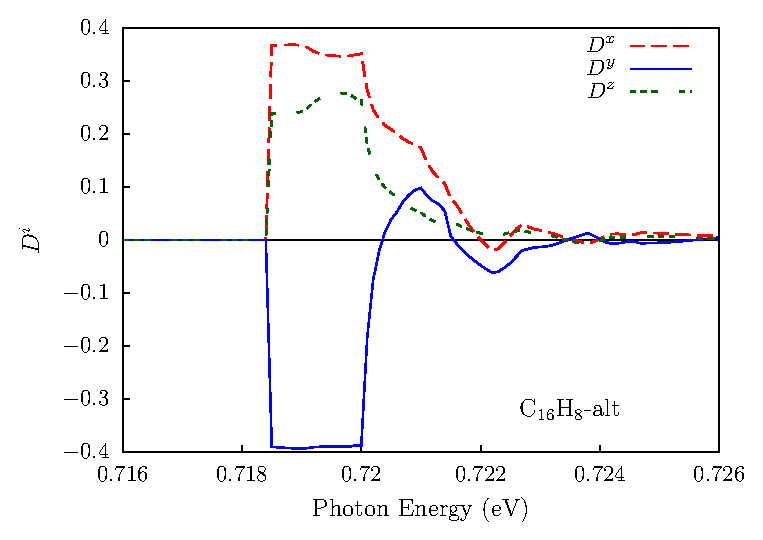
\includegraphics[width=\linewidth]{alt/alt-Da-final.eps}}
\hfill
\subfloat[]{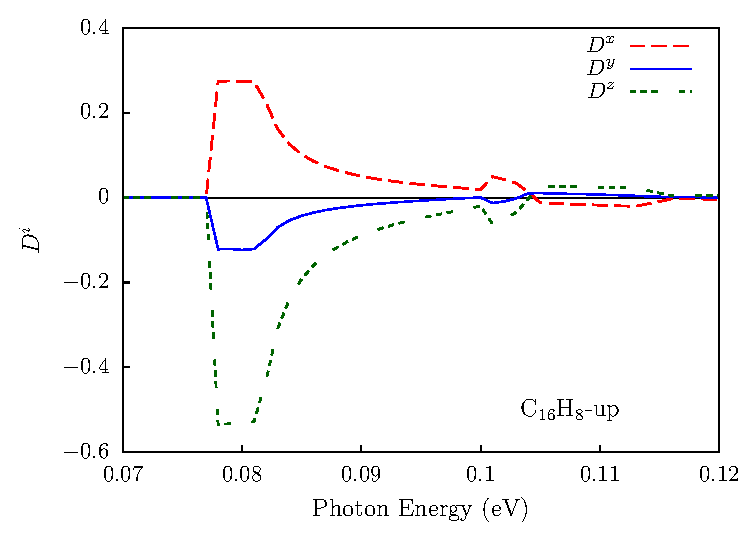
\includegraphics[width=\linewidth]{up/up-Da-final.eps}}
\caption{(Color online) Spectra of the degree of spin polarization along
    the \emph{i} direction, {$D^{i}$}, for the hydrogenated graphene structures
    C$_{16}$H$_{8}$-alt and C$_{16}$H$_{8}$-up under
    incidence of circularly polarized light.\label{fig:Da}}
\end{figure}

\begin{figure}[b]
\subfloat[]{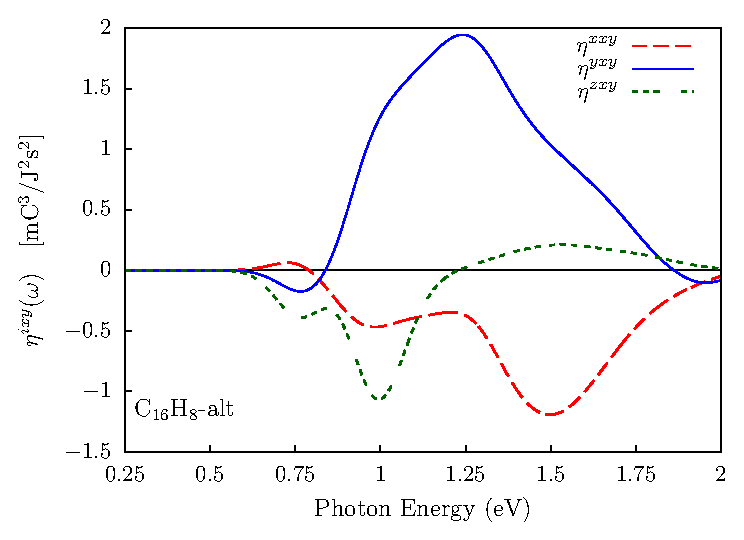
\includegraphics[width=\linewidth]{alt/alt-eta_sm-final.eps}}
\hfill
\subfloat[]{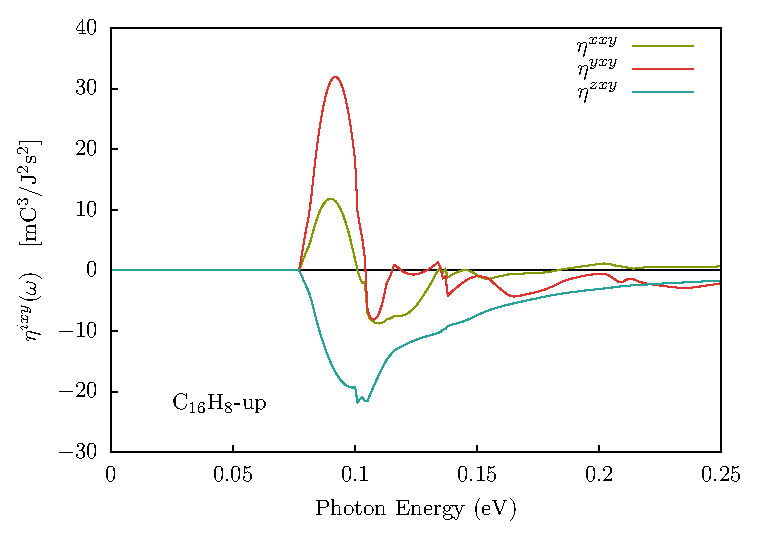
\includegraphics[width=\linewidth]{up/up_eta_kk_final.eps}}
\caption{(Color online) Spectra of the injection current tensor along the
     \emph{i} direction, {$\eta^{ixy}$}, for the hydrogenated graphene structures
    C$_{16}$H$_{8}$-alt and C$_{16}$H$_{8}$-up under incidence of circularly polarized light.\label{fig:eta}}
\end{figure}

\begin{figure}[t]
\subfloat[]{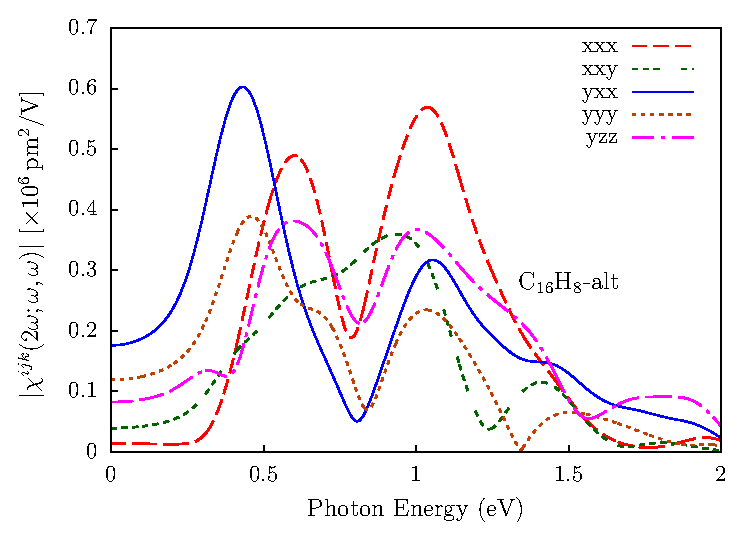
\includegraphics[width=\linewidth]{alt/alt_shg_final-abs_sm.eps}}
\hfill
\subfloat[]{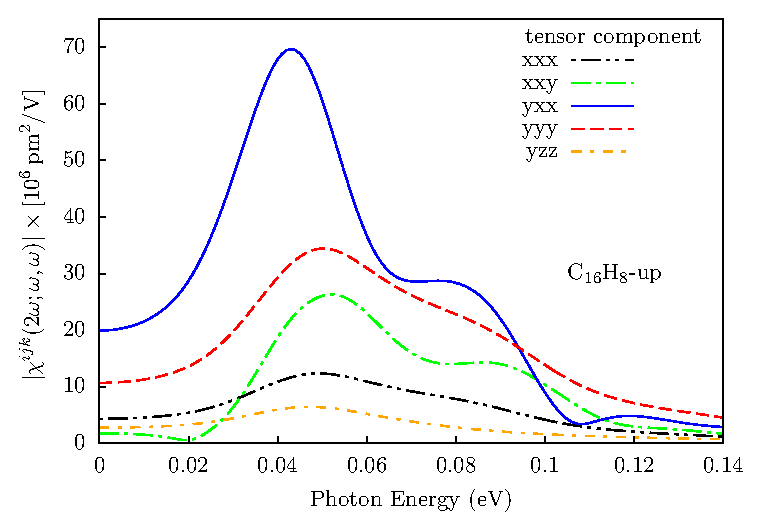
\includegraphics[width=\linewidth]{up/up_shg_final_abs_sm.eps}}
\caption{(Color online) Spectra of the absolute value of SHG for the C$_{16}$H$_{8}$-alt 
    and C$_{16}$H$_{8}$-up structures corresponding to the sum of the absolute 
    value for the non zero real and imaginary components of $\chi^{abc}(2\omega;\omega,
    \omega) $ tensor.\label{fig:shg-abs-both}}
\end{figure}



In Fig. \ref{fig:Da} we show the spectra obtained for
{$D^{i}$} of the C$_{16}$H$_{8}$-alt and C$_{16}$H$_{8}$-up structures. Values over
(under) zero define a positive (negative) direction of spin polarization along
the \emph{i} direction. 
For both structures the gap starts absorbing energy till the energy of the incoming light beam is major to it. For the \emph{alt} system it occurs near to 0.7185\,eV and for the \emph{up} one occurs near to 0.078\,eV of energy. 
It can be observed that for both structures we have
more than 30\% of {$D^{i}$} and a maximum absolute value in the \emph{y} direction,
reaching near to 60\% for the \emph{alt} case. 
Also it is important to mention that for both cases we have a range of energy in which is possible to hold the maximum DSP. 
The \emph{alt} structure presents a wide range of energy in which it is possible to have a 39\% of $D^{y}$.  It occurs from  0.7185 to 0.72\,eV of energy and a similar behavior is shown for the  $D^{x}$ and $D^{z}$ components for leaser values of DSP. After the energy of 0.72\,eV the DSP vanishes for the three components. The \emph{up} system presents a similar behavior from 0.078 to 0.081\,eV presenting a minimal variation in the $D^{y}$ component. Again, the $D^{x}$ and $D^{z}$ components have their own maximum values for this range of energy and after 0.081\,eV the DSP slowly vanishes to zero. In table \ref{tab:dacomp}we show a comparison of the maximum degree of spin polarization reported for different structures. As we can see from table the \emph{alt} and \emph{up} systems have leaser $D^{a}$ than the Si(111)-As 1$\times$1 and the the bulk CdSe system. The $D^{a}$ is comparable with the Si(111)-In 8$\times$2 bulk Si, and bulk GaAs systems for different photon energies where the maximum value of DSP is reached. This makes the use of light sources in another range of energy possible, having, as mentioned before, a wide range in which the maximum DSP is hold.

We show in Fig. \ref{fig:eta}
the spectra obtained for the current tensor {$\eta^{ixy}$} of the
\emph{alt} and \emph{up} systems, respectively. Again as in the case of DSP the gap starts absorbing the energy of the incident beam. We can observe that
circularly polarized light (CPL) on the plane $xy$ produces injection current
along three directions. Values over (under) zero define a positive (negative)
direction of current injection along the \emph{i} direction. From Fig.
\ref{fig:eta} we can see that for the \emph{alt} system spectra 
we have a positive maximum in the \emph{y} direction for an
incident beam energy of 1.25\,eV, reaching a value of
3.7\,mC$^{3}$/J$^{2}$s$^{2}$. Also, for the \emph{up} spectra 
we have a positive maximum in the \emph{y} direction for an
incident beam energy of 0.09\,eV, reaching a value of
28\,mC$^{3}$/J$^{2}$s$^{2}$. After 1.55 and 0.125\,eV of the incident field the photocurrent for the \emph{alt} and \emph{up} systems, respectively, smoothly decreases and later the response vanishes. In table \ref{tab:etacomp} we present a comparison
of the maximum current injection reported for different structures.
From the table we can see that, excluding the case of the bulk CdSd, the systems presented here have large values in comparison with the other systems. For the \emph{alt} structure this response is comparable wit the Si(111) 2$\times$1 system for a larger photon energy and the response for the \emph{up} structure has the same order of magnitude as the bulk CdSd both in this case for a lower energy of the incoming beam.

In Fig. \ref{fig:shg-abs-both}  we show the absolute value of the  spectra obtained
for the SHG of the \emph{alt} and \emph{up} systems when we evaluated the $
\chi^{abc}(2\omega;\omega\omega)$ tensor. We can see
that for the \emph{alt} structure an absolute
maximum of the SHG spectra is reached at 0.4\,eV with a value of
0.6$\times10^{6} $\,pm$^{2}$/V for the $\chi^{yxx} $ component produced
principally for contributions of the imaginary part. Also, a second local
maximum is reached at 1.1\,eV with a value of 0.55$\times10^{6} $\,pm$^{2}$/V
for the $\chi^{xxx} $ component having in this case a principal contribution
from the real part. In the other hand, we can see that for the
\emph{up} structure the absolute maximum is found near to 0.042\,eV reaching a
value of 70$\times10^{6} $\,pm$^{2}$/V for the $\chi^{yxx} $ tensor component
which contribution comes from the imaginary part of the spectra. In table
\ref{tab:shgcomp} we show a comparison of the maximum SHG reported for
different structures. From the table we can see that the \emph{alt} structure has the minimum absolute value of the SHG tensor while the \emph{up} has he biggest one. In both cases the energy of the incoming beam needed to produce SHG is smaller than for the other cases shown here.  


\begin{table}[htb]%
  \sidecaption
  \begin{tabular}{lcccc}
  \hline
  Structure & Energy &  \multicolumn{2}{c}{$D^{a}$} &  Ref.\\
  \cline{3-4}
  & [eV]   & component & [\%] \\
  \hline
  C$_{16}$H$_{8}$-alt  & 0.719& y & 39     & * \\
  C$_{16}$H$_{8}$-up   & 0.08 & y & 57     & * \\
  Si(111)-In $8\times2$& 0.74 & z & 32     & \cite{arzate2014optical}  \\
  Si(111)-As $1\times1$& 2.20 & z & 100    & \cite{mendoza2012optical} \\
  Bulk Si              & 3.44 & z & 30     & \cite{nastos2007full}     \\
  Bulk GaAs            & 1.50 & z & 50     & \cite{nastos2007full,bhat2005excitonic} \\
  Bulk CdSe            & 1.8  & z$^{\dag}$ & 100& \cite{nastos2007full}\\
  \hline
  \end{tabular}
  \caption[]{%
  Comparison of the reported absolute values for the highest 
  percentage of {$D^{i}$} for different structures.($^{*}$This work. $^{\dag}xy$ polarization)}
  \label{tab:dacomp}
\end{table}


\begin{table}[htb]%
  \sidecaption
  \begin{tabular}{lcccc}
  \hline
    Structure & Energy &  \multicolumn{2}{c}{$\eta^{a}$} &  Ref.\\
    \cline{3-4}
              & [eV]   & direction & [mC$^{3}$/J$^{2}$s$^{2}$] \\
    \hline
    C$_{16}$H$_{8}$-alt     & 1.25  & y & 3.70  & *     \\
    C$_{16}$H$_{8}$-up      & 0.09  & x & 28.0  & *     \\
    Si(111)-In $8\times2$   & 1.24  & y & 0.35  & \cite{arzate2014optical}  \\
    Si(111) $2\times1$      & 0.75  & y & 1.22  & \cite{mendoza2012optical} \\
    GaAs(110) clean         & 4.30  & y & 0.30  & \cite{nastos2007full}     \\
    GaS (110)-Sb            & 4.60  & y & 0.17  & \cite{cabellos2011optical}\\
    Bulk CdSd               & 1.8   & y$^{\dag}$ & 90.0  & \cite{nastos2006optical}  \\
  \hline
  \end{tabular}
  \caption[]{%
  Comparison of the highest reported absolute values of {$\eta^{ixy}$} for 
    different structures. ($^{*}$This work. $^{\dag}yz$ polarization)}
  \label{tab:etacomp}
\end{table}


\begin{table}[htb]%
  \sidecaption
  \begin{tabular}{lcccc}
  \hline
    Structure & Energy & \multicolumn{2}{c}{$\chi^{abc} $} &  Ref.\\
    \cline{3-4}
              & [eV]   & $abc$ & [$10^{6}$pm$^{2}$/V ] \\
    \hline
    C$_{16}$H$_{8}$-alt    & 0.4   & yxx   & 0.6   & *     \\
    C$_{16}$H$_{8}$-up     & 0.042 & yxx   & 70    & *     \\
    Si(100)2$\times$1      & 1.5   & xxx   & 1.5   & \cite{andersonPRB15} \ \\
    BN(6,0) NT pristine    & 5.0   & zzz   & 35    & \cite{salazar2014molecular} \\
    BN(6,0) NT+4(H$_{2}$)  & 5.0   & zzz   & 33    & \cite{salazar2014molecular} \\
    BN(6,0) NT+12(H$_{2}$) & 4.8   & zzz   & 15    & \cite{salazar2014molecular} \\
  \hline
  \end{tabular}
  \caption[]{%
  Comparison of the highest reported absolute values of SHG for 
    different structures and components. ($^{*}$This work.)}
  \label{tab:shgcomp}
\end{table}



%%%%%%%%%%%%%%%%%%%%%%%%%%%%%%%%%%%%%%%%%%%%%%%%%%%%%%%%%
%%%%%%%%%%%%%%%%%%%%%%%%%%%%%%%%%%%%%%%%%%%%%%%%%%%%%%%%%
%%               begin of conclusions section          %%
%%                                                     %%

\section{Conclusions} % (fold)
\label{sec:conclusions}

We have performed \emph{ab initio} calculations for the spin and current injection and
Second-Harmonic Generation (SHG) on the hydrogenated graphene C$_{16}$H$_{8}$-alt and
C$_{16}$H$_{8}$-up structures (Fig. \ref{fig:structures}) with the
independent particle approximation (IPA). Our calculations predicts that it is
possible to inject spin-polarized electrons along the perpendicular direction
to the surface plane, obtaining a degree of spin polarization (DSP) of the
injected electrons about 39\% and 57\%  (Fig. \ref{fig:Da}) at the photon energies of around 0.719
and 0.08\,Ha  for the \emph{alt} and \emph{up} cases, respectively. Also there is a range of energy
in which this DSP can be held, from 0.078 to 0.081\,eV and from 0.078 to 0.081\,eV for the \emph{alt} and \emph{up} cases, respectively. This results predicts that particularly the \emph{up} structure is usable for spintronics proposes. 
Also, our results about the optical current injection (OCI) with circularly polarized light (CPL)
show that the \emph{alt}  and \emph{up} systems have a response near to 3.70
and 28.0\,mC$^{3}$/J$^{2}$s$^{2}$ (Fig. \ref{fig:eta}) for incident beams with energies of around
1.25 and 0.09\,eV. According to measurements already done on bulk materials, it
is actually possible to measure such amount of injection current density. The motion of the electrons at the
C$_{16}$H$_{8}$-alt and C$_{16}$H$_{8}$-up structures can be controlled by the incidence of circularly
polarized light. Finally we found that the \emph{alt} and \emph{up} structures
present a absolute maximum of 0.6$\times 10^{6}$ and 70.0\,$\times 10^{6}
$\,pm$^{2}$/V (Fig. \ref{fig:shg-abs-both}) at the photon energies of around 0.40 and 0.042\,eV for the \emph{alt} and \emph{up} systems.
According to these results we can say that the \emph{up} system is usable for SHG.


\section{Acknowledgment} % (fold)
\label{sec:Acknouledgment}

This work has been supported by \emph{Consejo Nacional de Ciencia y
Tecnolog\'ia} (CONACyT), M\'exico, Grant No. 153930.


\bibliographystyle{pss}
\bibliography{graphane_structures}

\end{document}
